\documentclass{article}
\usepackage{titling}
\usepackage{lipsum}
\usepackage{amsmath}
\usepackage{listings}
\usepackage{graphicx}



\begin{document}
\noindent
\begin{minipage}[t]{0.6\textwidth}
    \begin{flushleft}
        \LARGE\textbf{Math 343 - Homework 1} \\
        \vspace{6pt} % add 6pt of vertical space
        \hrule width 10cm
        \vspace{12pt}
        \large\textbf{Preston Duffield} \\
        \large Western Washington University \\
        \today
        \vspace{24pt}
    \end{flushleft}
\end{minipage}


\section*{Question 1}

\subsection*{a)}
I would choose to test if the two population means where equal, ie,
\begin{flushleft}
    $H_0$: $\mu_1 = \mu_2$ \\
    $H_a$: $\mu_1 \neq \mu_2$ \\
\end{flushleft}
\subsection*{b)}
\begin{equation*}
    \begin{array}{c|c|c}
        & \text{Location 1} & \text{Location 2} \\
        \hline
        \text{Sample Mean} & \bar{y}_1 = 2980 & \bar{y}_2 = 3205 \\
        \text{Sample Standard Deviation} & S_1 = 1140 & S_2 = 963 \\
        \text{Sample Size} & n_1 = 40 & n_2 = 40 \\
        \text{Sample Variance} & S_1^2 = 1299600 & S_2^2 = 927369 \\
    \end{array}
\end{equation*}\\

At significance level $\alpha = 0.10$. With degrees of freedom $v = (n_1 + n_2) - 2 = 40 + 40 - 2 = 78$.

\begin{align*}
    S_p &= \frac{(n_1 - 1)S_1^2 + (n_2 - 1)S_2^2}{n_1 + n_2 - 2} \\
    &= \frac{(40 - 1) \times 129960 + (40 - 1) \times 927369}{40 + 40 - 2} \\
    &= 528664.5
    \end{align*}

\begin{align*}
    t &= \frac{y_1-\bar{y_2}}{S_p \sqrt{\frac{1}{n_1}+\frac{1}{n_2}}} \\
    &= \frac{2980 - 3205}{528664.5 \sqrt{\frac{1}{40}+\frac{1}{40}}} \\
    &\approx -0.0019
    \end{align*}

The Test Statistic $t_{\alpha / 2 , v} = t_{.05 , 78} \approx 1.671$. Note that $t < t_{.05 , 78}$ and is not in the critical region.
Therefore, there is not enough statistical evidence to support the population means being unequal, that is, $\mu_1 \neq \mu_2$. 

\subsection*{c)}
The P-value can be obtained in R using the following code.
\begin{lstlisting}[language=R, caption=Calculating the P-value for a $t$ value, basicstyle=\small]
    # define the t-statistic
    t <- -0.0019
    
    # calculate the P-value for a two-tailed t-test
    p_value <- 2 * pt(t, df = 78, lower.tail = FALSE)
    
    # print the P-value
    p_value
    \end{lstlisting}

The following code shows that the P-value $= 1.001511$.
\subsection*{d)}
A $90\%$ confidence interval for the difference in the true mean distance between
the two populations is:
interval for the difference in the true mean distance between
\begin{align*}
    (y_1-\bar{y}2)&\pm t{\frac{\alpha}{2}, 78} * S_p * \sqrt{\frac{1}{n_1} + \frac{1}{n_2}} \\
    &\pm 1.671 * 528664.5 * \sqrt{\frac{1}{40} + \frac{1}{40}} \\
    &\pm 197533.8
    \end{align*}
\begin{equation*}
    (-197785.8, 197308.8)
\end{equation*}
This confidence interval contains zero, which is consistent with conclusion reported above.

\section*{Question 2}

First we note that,
% t = (y-bar/mu_0)/S/root(n) is approximately N(0,1).
\begin{equation*}
    t = \frac{\bar{X} - \mu_0}{S/\sqrt{n}} \sim N(0,1)
    \end{equation*}
\begin{flushleft}
Then we can derive that,
    \end{flushleft}
    
    % As long as the sample size is sufficiently large and the population is normal or the sample size is very large, the statement is generally true by the Central Limit Theorem.
\begin{align*}
    1 - \alpha &= P(-t_{\alpha,n-1} \leq \frac{\bar{X} - \mu_0}{S/\sqrt{n}} \leq t_{\alpha,n-1}) \\
                &= P(-t_{\alpha,n-1} \frac{S}{\sqrt{n}} \leq \bar{X} - \mu_0 \leq t_{\alpha,n-1} \frac{S}{\sqrt{n}}) \\
                &= P(-\bar{X} - t_{\alpha,n-1} \frac{S}{\sqrt{n}} \leq -\mu_0 \leq -\bar{X} + t_{\alpha,n-1} \frac{S}{\sqrt{n}}) \\
                &= P(\bar{X} + t_{\alpha,n-1} \frac{S}{\sqrt{n}} \geq \mu_0 \geq \bar{X} - t_{\alpha,n-1} \frac{S}{\sqrt{n}}) \\
                &= P(\bar{X} - t_{\alpha,n-1} \frac{S}{\sqrt{n}} \leq \mu_0 \leq \bar{X} + t_{\alpha,n-1} \frac{S}{\sqrt{n}})
    \end{align*}

Therefore, the confidence interval for one population mean $\mu$ in the case
where the population variance $\sigma ^{2}$ is unknown can be described as

\begin{align*}
    \bar{X} \pm t_{\alpha,n-1}\frac{S}{\sqrt{n}}
\end{align*}

\section*{Question 3}
The P-value can be obtained in R using the following code, where $t_0$ varies.
\begin{lstlisting}[language=R, caption=Calculating the P-value for a $t_0$ value, basicstyle=\small]
    # Define the t_0 value, degrees of freedom, and tail of the distribution
    t_0 <- 2.48
    df <- 10
    tail <- 2
    
    # Calculate the P-value using the "pt" function
    p_val <- pt(t_0, df, tail)
    
    # Print the P-value
    print(p_val)
    \end{lstlisting}

\subsection*{a)}
When $t_0 = 2.48$, the P-value is $0.637$.
\subsection*{b)}
When $t_0 = 3.55$, the P-value is $0.869$.
\subsection*{c)}
When $t_0 = 2.00$, the P-value is $0.478$.

\section*{Question 4}

\subsection*{a)}

\begin{figure}[h]
    \centering
    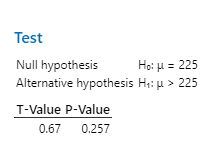
\includegraphics[width=0.5\textwidth]{./hw_1/images/4_b.png}
    \caption{The output of the 1-sample t test from Minitab.}
    \label{fig:4_a}
  \end{figure}
\begin{flushleft}
    $H_0$: The mean repair time is 225 hours. \\
    $H_a$: The mean repair time exceeds 225 hours.
\end{flushleft}
\subsection*{b/c)}
Since the p-value (0.257)
is greater than the significance level (0.05),
we fail to reject the null hypothesis. That is,
there is not enough statistical evidence to support that the mean repair
time exceeds 225 hours.
\subsection*{d)}
\begin{figure}[h]
    \centering
    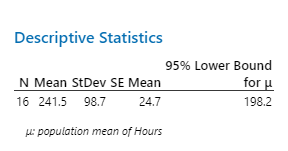
\includegraphics[width=0.5\textwidth]{./hw_1/images/4_a.png}
    \caption{The Descriptive Statistics of the 1-sample t test from Minitab.}
    \label{fig:4_b}
  \end{figure}



\section*{Question 5}

\subsection*{a)}
\subsection*{b)}
\subsection*{c)}
\subsection*{d)}
\subsection*{e)}

\section*{Question 6}

\section*{Question 7}
We can estimate the sample mean by observing the values at the $50^{th}$ percentile. This gives us:
$\stackrel{\sim}{\mu}= 98.6$\\
We can estimate the sample standard deviation by taking the reciprocal of the slope of the best-fit line.
This can be approximated as:
$\stackrel{\sim}{\sigma} = 1/0.27 = 3.7$\\
\end{document}
